% % % % % % % % % % % % % % % % % % % % % % % % % % % % % % % % % % % % % % % % 
% Formelsammlung von LaTeX4EI									
%
% @encode: 	UTF-8, tabwidth = 4, newline = LF
% @author:	Emanuel Regnath
% @date:		
%
% % % % % % % % % % % % % % % % % % % % % % % % % % % % % % % % % % % % % % % % 


%---------------------------------------%
%			P R E A M B L E				%
%~~~~~~~~~~~~~~~~~~~~~~~~~~~~~~~~~~~~~~~%

% Document Class ===============================================================
\documentclass[fs, footer]{latex4ei}

\usepackage{multirow}			% Spaltenpaket

\usepackage{tikz}				% Alle möglichen Zeichnungen

\sisetup{per-mode = fraction}
\titleformat{\subsubsection}{\normalsize\bfseries}{\thesubsubsection.\ }{0pt}{}

%---------------------------------------%
%			Nachrichtentechnik 			%
%~~~~~~~~~~~~~~~~~~~~~~~~~~~~~~~~~~~~~~~%

% DOCUMENT_BEGIN ===============================================================
\begin{document}

% Split in 4 Columns ===========================================================
\begin{multicols*}{4}

% TITLE ========================================================================
\fstitle{Nachrichtentechnik}

% Shanon: A Mathematical Theory of Communication 1948
\section*{Allgemeines}
\sectionbox{
\begin{center}
	\Fbox{Quelle} $\ra$ \Fbox{Sender} $\ra$ \Fbox{Kanal} $\ra$ \Fbox{Empfänger} $\ra$ \Fbox{Senke}\\[1em]
\end{center}

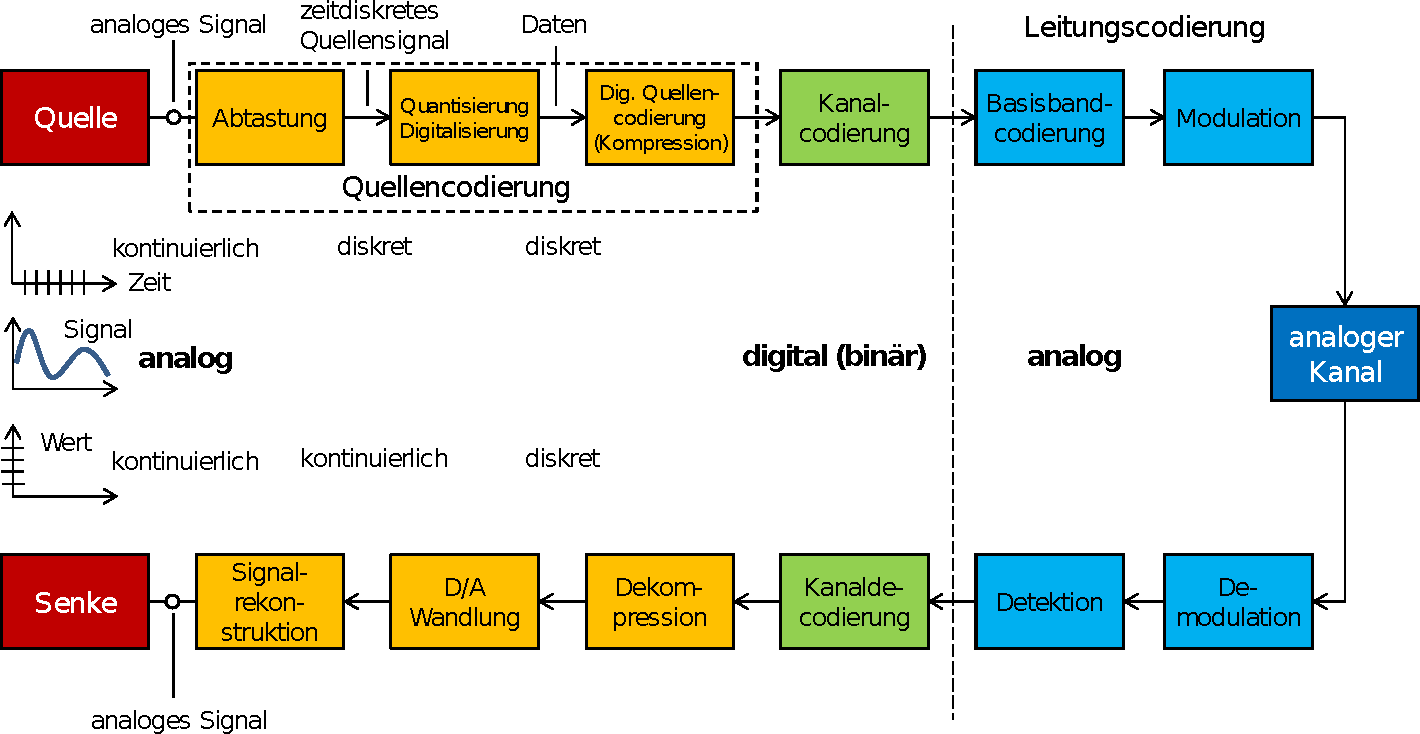
\includegraphics[width = \columnwidth]{./img/transmission.pdf}
Signal $\ra$ A/D Wandlung: Abtastung $\ra$ Digitaler Bitstrom $\ra$ D/A Wandlung: $\pm 1$ Gewichtete NF Impulse $\pm g_{\ir s}(t)$ $\ra$ Modulation: Verschiebung ins Trägerband $\ra$ AWGN Kanal $\ra$ Detektor $\ra$ Bitstrom


}

% SECTION ====================================================================================
\section{Signale}
% ============================================================================================
\sectionbox{
	\subsection{Arten von Signalen}
	\begin{description}
		\item[deterministisch:] durch Funktionen beschreibbar, enthalten kein Nachricht.
		\item[stochastisch:] zufälliger Verlauf, überträgt Information
	\end{description}
	
	
	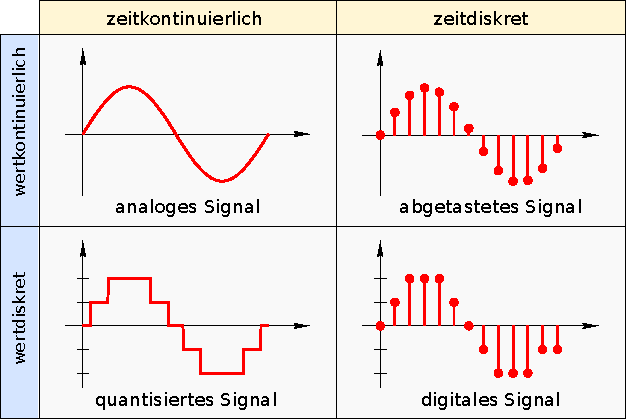
\includegraphics[width = \columnwidth]{./img/signals.pdf}

	Vorteile digitales Signal: Kompression, Verschlüsselung, Fehlerkorrektur
}


\sectionbox{
	\subsection{Sonstiges}
	Autokorrelation $r_{\textsf{V}}(\tau) \FT S_{\textsf{V}}(f)$ Leistungsdichtespektrum
	$x(t),y(t)$ sind orthogonal, falls $\int\limits_{-\infty}^\infty x(t)y(t) = 0$\\
	Kompl. Fehlerfunktion $\erfc(x) = 1 - \erf(x) = \frac{2}{\sqrt{\pi}} \int\limits_{x}^\infty e^{- \tau^2} \diff \tau$
}	


% SECTION ====================================================================================
\section{Abtastung von Signalen}
% ============================================================================================
\sectionbox{
\subsection*{Abtasttheorem}
Signal $x(t)$, Abtastfunktion $s(t) = T_A \sum \delta(t-nT_s)$, \\
Tiefpassfilter $h_r(t)$\\
\\
\begin{tabular*}{\columnwidth}{@{\extracolsep\fill}lll@{}}
	Vorgang & Zeitbereich & Frequenzbereich\\
	Abtasten: & $x_s(t) = s(t) \cdot x(t)$ & $X_s(\omega) = S(\omega) * X(\omega)$\\
	Rekonstr. & $x_r(t) = h_r(t) * x_s(t)$ & $X_r(\omega) = H_r(\omega) \cdot X_s(\omega)$\\
\end{tabular*}\\
\\
\begin{center} 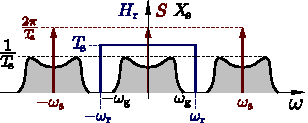
\includegraphics[scale = 1]{./img/sampletheorem.pdf} \end{center}

Bandbreite $\omega_g$, Abtastfrequenz $\omega_s$\\
\\
\boxed{ \omega_s = \frac{2 \pi}{T_s} \ge 2 \omega_g } \qquad \boxed{ \omega_g \le \omega_r \le \omega_s - \omega_g }

Abtastoperator: $\mathbb A\{x(t)\} = x(t) \cdot T_A \sum \limits_{n = - \infty}^{\infty} \delta (t - n T_A)$ \\
Rekonstruktion: $x_r(t) = T_{\ir A} \sum \limits_{n = - \infty}^{\infty} x(n T_{\ir A}) \cdot h_r(t - nT_{\ir A})$\\
Abbruchfehler: $\abs{\Delta} = \abs{\frac{x_r(t) - x(t)}{x(t)}}$\\
Periodisierungsoperator: $\mathbb P \{ X(f) \} = X(f) * \sum \limits_{n = - \infty}^\infty \delta (f - \frac{n}{T_A})$

Ideale Abtastung:
$\mathbb A \{x(t) \} \overset{f_A = 1 / T_A}{\ftsymbol} \mathbb P \{ X(f) \}$
}

%Projektion: $\int\limits_{-\infty}^{\infty} x(t) \sinc\left( \frac{t- nT_A}{T_A}\right) \diff t = T_{\ir A} x(n T_A)$\\
%$\int\limits_{-\infty}^{\infty} b_n(t) b_m(t) \diff t = \delta[m-n]$\\ 


%Sample\&Hold: Interpolation $\rightleftarrows$ Dezimierung\\



% SECTION ====================================================================================
\section{Quantisierung und Digitalisierung}
% ============================================================================================
wertkontinuierliche Sequenz von (zeitdiskreten) Abtastwerten wird abgebildet auf wertdiskrete Sequenz.
\begin{center}
 $x ( n T_A)$ mit $ n \in \mathrm Z$ $\overset{x_Q}{\longrightarrow} $ $x_Q (nT_A)$
\end{center} 

\sectionbox{
\subsection{Allgemeines}
Quantisierungsfunktion $\vec x_Q = \mathcal Q(\vec x)$

Bildet Vektoren $\vec x \in \R^N$ auf eine Menge $S$ ab mit $\abs{S} = M$

Man benötigt $m = \ceil{\log_2 M}$ bits um $\vec x_Q$ zu repräsentieren.\\
Intervall $I_i = [g_i, g_{i+1}]$ enthält Reprodwert $s_i$ \\

Skalare Quantisierer: $N=1$ \qquad Vektor Quantisierer: $N > 1$\\

Quantisierungsfehler: $\vec q (\vec x) = \vec x_Q - \vec x = s_i - x$

(besteht aus granularem Rauschen und Überlastungsrauschen)
}


\sectionbox{
	\subsection{Skalare Quantisierung $N = 1$}

	$m$ Bits für einen ($N = 1$) Abtastwert \\

	Quantisierungsfehler $q(x) = x_Q - x = x_Q (n T_A) - x (nT_A)$

	\emphbox{
		Quantisierungsfehlerleistung:

		$P_{\ir Q} = \int q(x)^2 f_{\X}(x) \diff x = \sum\limits_{s_i} \int_{g_i}^{g_{i+1}} (s_i - x)^2 f_{\X}(x) \diff x$ 
	}

	Optimales $s_i$ (setze $\frac{\partial P_Q}{\partial s_i} \overset{!}{=} 0$):

	$s_i = \frac{\int \limits_{g_i}^{g_{i+1}} x f_x (x) \diff x}{\int \limits_{g_i}^{g_{i+1}}  f_x (x) \diff x} = \E \left[ \X | x \in I_i \right]$
}


\sectionbox{
	\subsection{Lineare Quantisierung}
	Spezialfall der skalaren Quantisierung mit gleich großen Quantisierungsintervallen $\Delta$.
	
	\pbox{4cm}{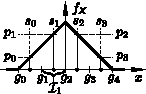
\includegraphics{./img/pdf_quantization.pdf}} \ \pbox{4cm}{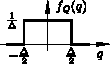
\includegraphics{./img/pdf_quantization_error.pdf}} \
	\pbox{4cm}{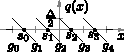
\includegraphics{./img/quantization_error.pdf}}\\
	\emphbox{Es gilt für PDF: $\int\limits_{-\infty}^\infty f_{\X}(x) \diff x \stackrel{!}{=} 1$}
	
	Gleich große Quantisierungsintervalle $\mathcal I_i=[g_i, g_{i+1}]$ mit Breite $\Delta$\\
	$\Delta = \frac{x_{\max} - x_{\min}}{2^m} = g_{i+1} - g_i$\\ 
	
	Reproduktionswerte $s_i$ in der Mitte der Intervalle (midriser)\\
	$s_i = \frac{2i - M + 1}{2} \Delta$\\ 
	
	Auftrittswahrscheinlichkeit $p_i$ der Quantisierungsstufe $s_i$ \\
	$p_i=\int_{g_i}^{g_{i+1}}f_{\ir X}(x)\diff x$\\

	\emphbox{Signalleistung $P_{\ir X} = \E[\X^2] = \int\limits_{x_{\min}}^{x_{\max}} x^2 f_{\X}(x) \diff x$}\\
	Gleichverteilung: $P_{\ir X} = \frac{x_{\max}^2}{3}$ \qquad Sinusförmig: $P_{\ir S} = \frac{x_{\max}^2}{2}$\\[1em]
	\emphbox{Fehlerleistung $P_{\ir Q} = \E[\textit{Q}^2] = \int\limits_{-\infty}^{\infty} q(x)^2 f_{\textit{Q}}(q) \diff q$}\\
	Bei gleichverteiltem Quantisierungsfehler: $P_{\ir Q} = \frac{\Delta^2}{12}$

	% wichtige Formel vgl. Übung 10 $P_Q = \sum \limits_{s_i} \int \limits_{-\Delta / 2}^{\Delta / 2} z^2 f_X (z + s_i) \diff z$

	\emphbox{Signal-Noise-Ratio: $\SNR_Q = \frac{P_{\ir X}}{P_{\ir Q}}$}
	$\SNR_Q = \frac{P_{\ir X}}{P_{\ir Q}} = \begin{cases}
		\frac{x^2_{\ir max} /3}{\Delta^2 / 12} = 2^{2m} &\text{ bei gleichverteiltem Signal }\\
		\frac{x^2_{\ir max} /2}{\Delta^2 / 12} = \frac 3 2 2^{2m} &\text{ bei sinusförmigem Signal }\\
	\end{cases}$\\ \\
	Signal zu Quantisierungsrauschabstand $\SNR_{Q\si{\decibel}}$\\
	$\SNR_{Q\si{\decibel}} = 10 \log_{10}(\SNR_Q)\si{\decibel} = m \cdot \SI{6}{\decibel}$\\
	 (CD, $\SI{16}{bit}: \SI{96}{\decibel})$	
}


\sectionbox{
	\subsection{Nichtlineare Quantisierung}
	A-law-Kennlinie (Europa) und $\mu$-law-Kennlinie (USA)\\
	$C(x) = \begin{cases} \frac{A}{1 + \ln(A)} \cdot \abs{x} \cdot \sgn(x) & 0 \le \abs{x} \le \frac{x_{\max}}{A} \\[1em]
	\frac{1 + \ln\left( \frac{A \cdot \abs{x}}{x_{\max}} \right)}{1 + \ln(A)} \cdot \abs{x} \cdot \sgn(x) & \text{sonst} \end{cases}$

	$A = 87.5 = \SI{24}{\decibel}$

		\subsubsection{Pulse Coded Modulation PCM}
		Abtastung + skalare Quantisierung: $\SNR_Q = \frac{P_X}{P_Q} = 2^{2m}$
	
		\subsubsection{Differentielle PCM (DPCM)}
		Differenz zu vorhergesagtem Wert wird quantisiert.\\
		Prädiktion 0.ter Ordnung: Kann bei schnellen, großen Änderungen nicht mehr folgen.
		Gut geeignet für Signale mit hoher zeitlicher Konzentration $\ra$ schmales Spektrum.

		\subsubsection{Delta-Modulation (Hohe Überabtastung)}
		1-Bit-Quantisierung: $e_Q(nT_{\ir S}) = \pm \Delta$\\
		Kann den Wert nicht Konstant halten, Tiefpass am Empfänger nötig

		\subsubsection{Sigma-Delta-Modulator}
		$\sum$: Summe/Integral \qquad $\Delta$: 1-bit-Quantisierer
}


\sectionbox{
	\subsection{Optimale skalare Quantisierung}
	\cookbox{Lloyd-Max-Algorithmus}{
		\item Wähle Startwerte für alle $s_i^{(0)}$
		\item Intervallgrenzen: $g_i^{(t+1)} = \frac{ s_i^{(t)} + s_{i-1}^{(t)} }{2}$  \qquad $i = 1, \ldots , M-1$
		\item Reprod. Werte: $s_i^{(t+1)} = \E[\X | \X \in I_i]$ \quad\ $i = 0, \ldots , M-1$
		\item Fehlerleistung $P_Q^{(t+1)} = \E[Q^2]$ mit $s_i^{(t+1)}$ und $g_i^{(t+1)}$
		\item Berechne relative Änderung $\delta^{(t)} = \frac{P_Q^{(t+1)}-P_Q^{(t)}}{P_Q^{(t)}}$
	}
}



\sectionbox{
	\subsection{Informationsgehalt und Entropie}
	Info vom Symbol $s_i$: $I_i = - \log_2 \P(\X_Q = s_i) = -\log_2 p_i$\\ 
	Entropie von $\X_Q$: $H(\X_Q) = \E[I] = - \sum\limits_{i = 0}^{M-1} p_i \log_2 p_i $
	$\left[\frac{\ir{bit}}{\ir {Symbol}}\right]$\\
	
	Mittlere Codewortlänge $\overline l = \E[l] = \sum \limits_{i= 0}^{n-1} p_i l_i$

	Die minimale mittlere Codewortlänge $\overline l \ge H(x_Q)$
}

% SECTION ====================================================================================
\section{Codierung}
% ============================================================================================
	Komprimierung: Falls Bitstrom nicht gleichverteilt und mit Gedächtnis\\
	Maximale Kompression: Bits gleichverteilt, ohne Gedächtnis\\
	Entropie: kein Code kann für $\Z$ eine geringere mittlere Codewortlänge finden als $H(z) = \sum \P(z) \ld\left(\frac{1}{\P(z)}\right)$\\
\sectionbox{
	\subsection{Kompression}
	Kleiner Verlust bei unkodierten Bitstrom. Großer Gewinn bei Kodierung.\\
	Bsp: Feste Blocklänge mit Statusbit am Anfang: Kodiert/Unkodiert\\
}

\sectionbox{	
	\subsection{Digitale Quellencodierung (Kompression)}
	Arten von Kodierern:
	\begin{description}
		\item[Verteilung Bekannt:] Huffman Code, Morse, Arithmetic
		\item[Universal:] Lempel-Ziv (ZIP), PPM, BWT(bZip)
		\item[Transform:] Fouriertransformation (JPG,GIF,PNG,MP3)
	\end{description}
	%Kompression, Vektorquantisierung (verlustbehaftet) 
}

\sectionbox{

	\subsection{Kanalcodierung}
	Single-Parity-Check: 1 Bit pro 2 bit zusätzlich: XOR$(x_1,x_2)$\\
	Daraus ergibt sich eine Effizienz von $\frac{2}{3}$\\
	\\
	FEC: Forward Error Correction liefert Fehlererkennung und Korrektur.\\
	Beispiele: Paritätsbit, CRC, Reed-Solomon-Codes, LDPC,  Polar Codes
	
	% Paper Award IEEE: Polar Codes
	% Kanal lässt bestimmte Frequenzen durch: Luft hat bei 60GHz ein Minimum weil Wassermoleküle dagegen schwingen.
}

\columnbreak
% SECTION ====================================================================================
\section{Basisbandübertragung}
% ============================================================================================
%PAM: Puls-amplituden-modulations-verfahren\\

%	Wie wählt man $g(t)$?\\
%	Ressourcen: Zeit, Bandbreite, Energie, (Raum)\\


\sectionbox{
	\subsection{Impulsformen}
		\subsubsection{Rechteckimpuls $\rect\left(\frac{t}{T}\right)$:}
		$g_{\ir NRZ}(t) = \begin{cases}
			1, &\text{ für } \abs{t} < \frac T 2 \\
			\frac 1 2, &\text{ für } \abs{t} = \frac T 2 \\
			0, &\text{ sonst }			
		\end{cases}$
		\hfill $G_{\ir NRZ}(f) = T \sinc (fT)$\\ %T \frac{\sin(\pi f T)}{\pi f T}
		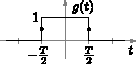
\includegraphics{./img/FT/NRZ_t.pdf} \hfill  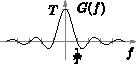
\includegraphics{./img/FT/NRZ_f.pdf}

		\subsubsection{Manchester Impuls:} 

		$g(t) = - g_{\ir NRZ} (t) + 2 g_{\ir NRZ} (2 t) = \begin{cases}
			1, &\text{ für } \abs{t} < \frac T 4 \\
			0, &\text{ für } \abs{t} = \frac T 4 \\
			-1, &\text{ für } \frac T 4 < \abs{t} < \frac T 2 \\
			- \frac{1}{2},  &\text{ für } \abs{t} = \frac T 2 \\
			0, &  \text{ sonst } \\
		\end{cases}$

		$G(f) = T \left( \frac{\sin ( \pi f \frac T 2 )}{\pi f \frac T 2 } - \frac{\sin ( \pi f T)}{\pi f T}\right)$ % = T(\sinc(fT/2) - \sinc(fT))$

		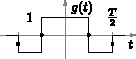
\includegraphics{./img/FT/manchester_t.pdf} \hfill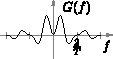
\includegraphics{./img/FT/manchester_f.pdf}

		Mittelwert Null, kein Gleichanteil
		\subsubsection{$\cos^2$-Impuls:} 
		$g(t) = \begin{cases}
			\cos^2\left(\frac{\pi t}{T}\right), &\text{ für } \abs{t} < \frac{T}{2}\\
			0, & \text{ sonst }
		\end{cases} $
		

		$G(f) = \frac{T}{2} \frac{\cos(\pi f \frac{T}{2})}{1 - (fT)^2} \frac{\sin (\pi f \frac T 2)}{\pi f \frac T 2}$

		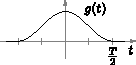
\includegraphics{./img/FT/cos2_t.pdf} \hfill 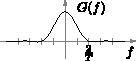
\includegraphics{./img/FT/cos2_f.pdf}

		\subsubsection{$\sinc$-Impuls: $\sinc(x) = {\rm si}(\pi x)$}
		$g(t) = \frac{\sin (\pi \frac t T)}{\pi \frac t  T} = \sinc\left(\frac{t}{T}\right)$ \hfill
		$G(f) = \begin{cases}
			T, &\text{ für } \abs{f} < \frac{1}{2T}\\
			\frac T 2 , &\text{ für } \abs{f} = \frac{1}{2T}\\
			0, &\text{ sonst } \\
		\end{cases}$

		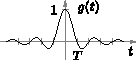
\includegraphics{./img/FT/sinc_t.pdf} \hfill 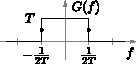
\includegraphics{./img/FT/sinc_f.pdf}
		\subsubsection{„Nyquist roll-off“-Impuls:}

		$g(t) = \frac{\sin (\pi \frac t  T)}{\pi \frac t  T} \cdot \frac{\cos (\alpha \pi \frac t T )}{1 - 4 \alpha^2 (\frac t T )^2}$

		$G(f) = \begin{cases}
			T &\text{für} \abs{f} \le \frac{1 - \alpha}{2T} \\
		\frac{T}{2} [ 1 + \cos ( \frac{\pi T}{\alpha} ( \abs{f} - \frac{1 - \alpha}{2T}) ) ] &\text{für} \frac{1 - \alpha}{2T} < \abs{f} \le \frac{1 + \alpha}{2T} \\
			0 & \text{sonst} 
		\end{cases}$

		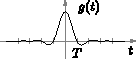
\includegraphics{./img/FT/nyquist_t.pdf} \hfill 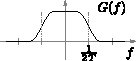
\includegraphics{./img/FT/nyquist_f.pdf}

		\subsubsection{Root-Raised-Cosine:}
		Meist genutzer Filter (Wurzel-Nyquist)
		\subsubsection{Gauß-Impuls:}
		$g(t) = \exp\left[ -\pi\left( \frac{t}{\Delta t} \right)^2 \right]$

		$G(f) = \Delta t \cdot \exp \left(  - \pi \left(\Delta t f \right)^2 \right) = \frac{1}{\Delta f} \exp \left(- \pi \left( \frac{f}{\Delta f} \right)^2 \right)$
		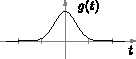
\includegraphics{./img/FT/gauss_t.pdf} \hfill 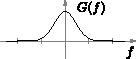
\includegraphics{./img/FT/gauss_f.pdf}
}

\columnbreak

% TODO: Skript Seite 56 + FT von Aufgabe 18a) von SUM D_n d(t-nT) --> SUM D_n e^(-j2Pi n f T)
	
\sectionbox{
	\subsection{Energie wichtiger Impulse mit Amplitude $A$}
	\begin{tabular}{@{}ll}
	$E_{S}\{\rect(\frac{t}{\alpha T})\} = A^2 \alpha \abs{T}$ & $E_{S}\{\tri(\frac{t}{\alpha T})\} = \frac{2}{3} \alpha \abs{T} A^2$\\
	$E_{S}\{\sinc(\frac{t}{\alpha T})\} = A^2 \abs{\alpha} \abs{T}$ & Rampe 0 bis $\alpha T$: $\frac{\alpha}{3} \abs{T} A^2$\\
	\end{tabular}
}


\sectionbox{	
	\subsection{Bandbreite}
	Absolut: Alle positiven Frequenzen\\
	B$_{99}$ Bandbreite: 99\% der Signalenergie bzw. -leistung liegen in diesem Bandbreitenbereich (geht auch mit 90\%)\\
	B$_{\ir 6dB}$ Bandbreite: Bis Hälfte des Spektrums $G(f)$\\
	B$_{\ir 3dB}$ Bandbreite: Bis Hälfte der Leistung\\
	B$_N$ Äquivalente Rauschbandbreite\\
	
	Bandbreiteneffizienz (Effizienz des Modulationsverfahrens):

	$\eta = \frac{\text{Übertragungsrate}}{\text{NF Bandbreite}}$ \qquad $\unitof{\eta} = \frac{\si{bit/s}}{\si{\hertz}}$

	Beispiel GSM: $\eta = 0.88 \frac{\si{bit/s}}{\si{\hertz}}$, \quad LTE: $\eta = \frac{3 \si{Gbit/s}}{100 \si{\mega \hertz}} = 30 \frac{\si{bit/s}}{\si{\hertz}}$\\
}


\sectionbox{
	\subsection{Frequenz-Zeit-Unschärfe}
	\emphbox{Ein Signal kann nicht gleichzeitig hart Band- und Zeitbegrenzt sein!\\
	\textbf{Unschärfe:} $T_D \cdot B_0 \ge \frac{1}{4\pi}$ }
	%$E = \int\limits_{-\infty}^\infty g^2(t) \diff t = \int\limits_{-\infty}^\infty \abs{G(f)}^2 \diff f$\\
	%Bandbreite: $B_0^2 = \frac{1}{E} \int\limits_{-\infty}^\infty f^2 \abs{G(f)}^2 \diff f$\\
	%$T_D^2 = \frac{1}{E} \int\limits_{-\infty}^\infty t^2 \abs{g(t)}^2 \diff t$\\
	Nach Trägheitsradius definiert. (Integral $\int\limits_{-\infty}^\infty t^2 g_{\ir s}^2 \diff t$ konvergiert)

	\textbf{Schrankenfunktion für Spektrum:}\\
	Falls das Zeitsignal in der $n$-ten Ableitung das \emph{erste} mal einen Sprung aufweist, gilt für das Betragsspektrum:\\
	\emphbox{ $\displaystyle \abs{X(f)} \propto \frac{1}{\abs{f}^{n+1}}$ \qquad für große $\abs{f}$}\\
	Anmerkung: $n$ kann auch negativ sein! Bsp: $\dirac(t) \Ra n = -1$
}

\sectionbox{
\subsection{Nyquist Bedingungen}
	\subsubsection{1. Bedingung: Kein Symbolübersprechen}
	Impulsantwort $g[nT] = \begin{cases} 1 & n = 0 \\ 0 & n \ne 0 \end{cases}$\\
	Fordert maximale vertikale Öffnung des Auges\\
	Impuls Nullstellen: $\pm 1T, \pm 2T, \pm 3T, \ldots$\\

	Zeitbereich: $A \{ g(t) \} = T \sum \limits_{n = - \infty}^{\infty} g(nT) \cdot \delta (t - nT) = T \cdot \delta (t)$
	Frequenzbereich: $P \{ G(f) \} = \sum \limits_{k = - \infty}^{\infty} G(f - \frac{k}{T}) = T$

	\subsubsection{2. Bedingung: Verschärfung 1. Bedingung}
	Impulsantwort $g \left[k \frac{T}{2}\right] = \begin{cases} 1 & k = 0 \\ g\left[\frac{T}{2}\right] & k = \pm 1 \\ 0 & \text{sonst} \end{cases}$\\
	Fordert maximale horizontale Öffnung des Auges\\
	Zusätzliche Impuls Nullstellen: $\pm 1.5T, \pm 2.5T, \pm 3.5T, \ldots$\\
}


\sectionbox{
\subsection{Augendiagramm}
\pbox{3cm}{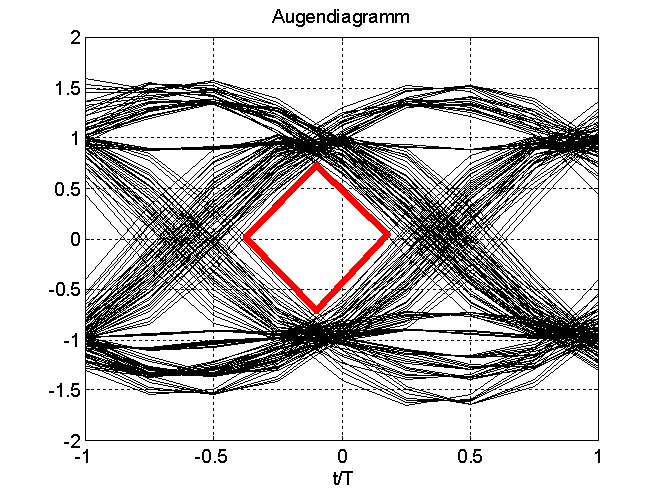
\includegraphics[width = 2.5cm]{./img/auge3.jpg}}
\pbox{4cm}{Bestimmung des Augendiagramm (4 Durchläufe): Für die Bereiche $[-T_{\ir A},0]$ und $[0,T_{\ir A}]$ werden die relevanten Pulse
so überlagert(positiv oder negativ), dass das Auge minimal wird. Daraus ergibt sich die Überlagerungstabelle.}\\

\parbox{2.5cm}{Beispiel mit \\ 1 Vor- und 2 Nachläufern:}
\tabcolsep0.5em
\begin{tabular}{lll|lll}
$D_{-2}$ & $D_{-1}$ & $D_{1}$ & $\boldsymbol D_{-1}$ & $\boldsymbol D_{1}$ & $\boldsymbol D_{2}$\\
$+1$ & $-1$ & $-1$ & $-1$ & $-1$ & $+1$\\ \mrule
$-1$ & $+1$ & $+1$ & $+1$ & $+1$ & $-1$\\
\end{tabular}

\begin{description}
	\item[Vertikale Öffnung $A_v$:] Maß für Empfindlichkeit gegenüber Rauschen
	\item[Horizontale Öffnung $A_h$:] Maß für Empfindlichkeit gegenüber Schwankungen des Abtastzeitpunkts
\end{description}
}





\sectionbox{
\subsection{Korrelation}
Ein Maß für die Ähnlichkeit zweier Signale $x(t), y(t)$ bei Verschiebung.\\
Korrelationskoeffizient $\rho_{xy} = \frac{E_{xy}}{\sqrt{E_x \cdot E_y}} = \frac{\varphi_{xy}(0)}{ \sqrt{\varphi_x(0) \cdot \varphi_y(0)}}$\\
\\
Es gilt: Korreliert $\rho = 1$, Orthogonal $\rho = 0$, Antipodisch $\rho = -1$\\
\\
\textbf{Kreuzkorrelationsfkt.} zwischen zueinander verschobenen Signalen:\\
	\emphbox{ $\displaystyle \varphi_{xy} (\tau) =  \varphi_{yx}(-\tau) = \int\limits_{-\infty}^{\infty} x(t) \cdot y(t+\tau) \diff t$ }
	Zusammenhang mit Faltung: $\varphi_{xy} (\tau) = x(-t) * y(t)|_{t = \tau}$\\
	\\
\textbf{Autokorrelationsfkt. AKF} ist Kreuzkorrelation mit sich selbst ($y = x$):\\
$\varphi_x (\tau) = \varphi_{xx}(\tau)$ \qquad Anwendung: Erkennen von Perioden\\ 
\\
\textbf{Energiebeziehung:} $E_{x,y} = \rho_{x,y} \sqrt{E_x E_y}$ mit \\
\textbf{Energie} $E_x = \int\limits_{- \infty}^{\infty} x(t)^2 \diff t = \int\limits_{- \infty}^{\infty} \Phi_x \diff f = \varphi_{xx}(0)$ \quad (endl. Sig.)\\
\textbf{Leistung} $P_x = \E[\X^2] = \frac{1}{2T} \int\limits_{-T}^{T} x(t)^2 \diff t$ \qquad\qquad (period. Sig.)\\
\textbf{Leistungsdichtespektrum} $\Phi_x(f)$ ist definiert als $\varphi_x \FT \Phi(f)$\\

Periodische Signale: $\overline \varphi_{xy}(\tau) = \frac{1}{2T} \int_{-T}^{T} x(t) y(t+\tau) \diff t$\\
\textbf{Stochastische Signale:} $\varphi_{\X\Y}(\tau) = \E[\X(t) \cdot \Y(t+\tau)]$\\
$\rho_{\X,\Y} = \frac{\Cov[\X \Y]}{\sigma_{\X} \sigma_{\Y}}$\\
$\int \limits_{-\infty}^{\infty} \PSD_{\X}(f) \diff f = \ACF_{\X}(0) = \Var[\X] + \E[\X]^2 = \sigma^2_{\X} + \mu^2_{\X}$
}




% SECTION ====================================================================================
\section{Analoger Übertragungskanal}
% ============================================================================================


$r(t) = h(t) * s(t)$ \qquad $R(f) = H(f) \cdot S(f)$\\ 
Verzerrungsfrei: $h(t) = h_0 \dirac(t-t_0)$ \qquad $H(f) = h_0 e^{-\i 2 \pi f t_0}$


\sectionbox{
	\subsection{\textsc{AWGN} -- Additive White Gaussian Noise}
	Weißes Rauschen $\textit{N}$ enthält alle Frequenzen. Thermisch: $N_0 = k_{\ir B} T$\\
	\begin{tabular}{lll}
	PDF & $f_\textit{N}(n) = \frac{1}{\sqrt{2\pi} \cdot \sigma} e^{-\frac{n^2}{2\sigma^2}}$\\[0.5em]
	LDS: & $\Phi_\textit{N}(f) := \frac{N_0}{2}$ &für $f < \SI{10}{\giga \hertz}$\\[0.5em]
	AKF: & $\varphi_n(\tau) = \frac{N_0}{2} \delta(\tau)$ & $\Ra 0$ für $\tau \ne 0$\\[0.5em]
	Leistung & $P_\textit{N} = \int \Phi_\textit{N} \diff f = \sigma^2 = B \cdot N_0$\\
	\end{tabular}

	Äquivalente Rauschbandbreite $B_N$: Bandbreite eines idealen Tiefpasses, der die selbe Rauschleistung $P_N$ erzeugt, 
	wie das reale Tiefpassfiltersystem.
}




% SECTION ====================================================================================
\section{Detektion im Rauschen}
% ============================================================================================
\sectionbox{
	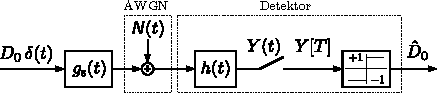
\includegraphics[width = \columnwidth]{./img/detection.pdf}

	gewähltes Bit $\hat D_n$ eines tatsächlichen Bits $D_n = \eset{1,0}$\\
	Ziel: $\P(\hat D_n \ne D_n)$ soll minimal sein.\\
	Lösung: maximiere SNR zum Abtastzeitpunkt $nT$\\
	Rauschleistung nach Filterung mit $h(t)$:\\
	$P_\textit{N} = \int\limits_{-\infty}^\infty \Phi_\textit{N} \abs{H(f)}^2 \diff f = \frac{N_0}{2} \int\limits_{-\infty}^\infty \abs{H(f)}^2 \diff f$ 

	$\ra $ mit Satz von Parseval gilt : $ P_{\ir N} =  \frac{N_0}{2} \int\limits_{-\infty}^{\infty} \abs{ h(t)}^2 \diff t$

	momentane Signalleistung: $P_s(t) = \abs{y_s(t)}^2$

	mittlere Signalleistung: $P_s = \lim\limits_{T \rightarrow \infty} \frac{1}{2T} \int\limits_{-T}^{T} \abs{y_{s}(t)}^2 \diff t$

}

\sectionbox{
	\subsection{Matched Filter}
	Signalangepasster Filter damit Signal im AWGN Kanal zum Abtastzeitpunkt die maximale SNR hat.
	Impulsantwort des Matched Filters:\\ $h_{\ir MF}(t) = K \cdot \cxc g_s(T-t)$ \qquad (entspricht gewendetem Sendeimpuls)\\
	$H_{\ir MF}(f)=K\cdot \cxc G_s(f)\cdot \e^{-\j 2\pi f T}$\\
	Maximum SNR: $\frac{P_s}{P_N} = \frac{2E_s}{N_0}$\\
}

\sectionbox{
	\subsection{Fehlerwahrscheinlichkeit $\P_b$}
	% Alle Pulse mit gleicher Energie haben die gleiche Fehlerwahrscheinlichkeit?
	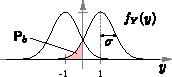
\includegraphics[width = 4cm]{./img/noisedetection.pdf}\\
	$\P_b = \frac{1}{\sqrt{2 \pi}} \cdot \int_{z_0}^\infty e^{\frac{-z^2}{2}} \diff z = Q(z_0) = \frac{1}{2} \erfc\left(\sqrt{\frac{1}{2} \SNR}\right)$\\
	Substituiere $z_0$\\
	Für matched Filter: $\P_b = Q(\sqrt{P_s / P_n}) = Q(\sqrt{Y_s^2 / \sigma_N^2}) = Q(\sqrt{2 E_s / N_0}) = Q(\sqrt{\SNR})$
}

\sectionbox{	
	\subsection{Zeitdiskreter AWGN-Kanal}
	$\sigma^2 = \frac{\sigma_\textit{N}^2}{A^2} = \frac{N_0}{2 E_s} = \frac{1}{\SNR}$\\
}

\sectionbox{	
	\subsection{Unabhängiges (unkorreliertes) Rauschen}
	Falls die erste Nyquistbedingung erfüllt und maximale SNR: \\ $\Ra$ Die Folge abgetasteter Rauschanteile ist unabhängig!
}



% SECTION ====================================================================================
\section{Lineare, digitale Modulation}
% ============================================================================================
\sectionbox{
\subsection{Allgemeines}
	Dimensionen: Phase (sin/cos), Polarisation (hori/vert)

	Die meisten Medien übetragen um eine Trägerfrequenz $f_0$ (Bandpass)\\

	Bandpass-Sendesignal (moduliert mit $S(t)$): \\ 
	$\tilde S(t) = A(t) \sqrt{2} \cos\left(2 \pi (f_0+F(t)) t + \varphi_0(t)\right)$\\

	Inphasenanteil (Cosinusträger) $S_I(t) = A(t) \cos(\varphi'(t))$

	Quadraturanteil (Sinusträger) $S_Q(t) = A(t) \sin(\varphi'(t))$

	Amplitude: $\abs{A(t)} = \sqrt{S_I^2(t) + S_Q^2 (t)}$

	Phase: $\varphi' (t) = \arctan \frac{S_Q (t)}{S_I (t)}$
	
	Mittl. Energie pro Symbol: $\ol E_S = \E[D_{I_n}^2 + D_{Q_n}^2] \cdot \underbrace{\int_0^T \abs{g_s (t)}^2 \diff t}_{E_{g_s}}$
	
	Energie je Bit : $\frac{E_s}{\text{Anzahl Bits}}$

	$d_{\ir min} $: Anfälligkeit gegenüber Rauschen
}

\sectionbox{
	\subsection{Modulation und Signalraumzuordnung}

	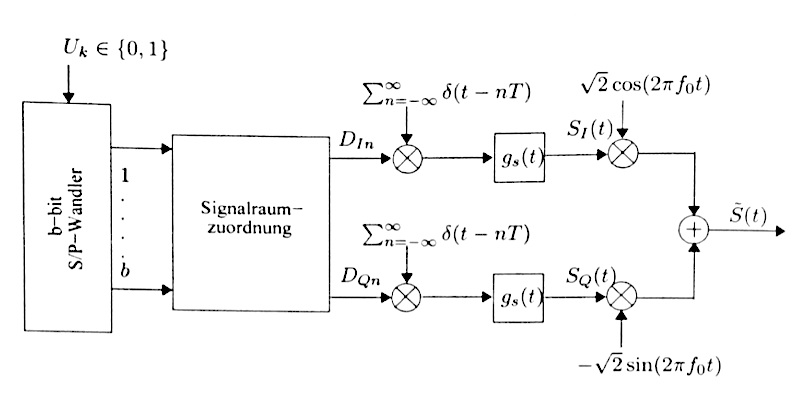
\includegraphics[width=6cm]{img/QAM_Sender.jpg}

	Moduliertes Sendesignal

	$\tilde S (t) = S_I (t) \sqrt{2} \cos (2 \pi f_0 t) - S_Q (t) \sqrt{2} \sin (2 \pi f_0 t) $ \\
	$= \left[ \sum \limits_{n = - \infty}^{\infty} D_{I_n} g_s (t - n T) \right] \sqrt{2} \cos (2 \pi f_0 t)$\\
	$-  \left[ \sum \limits_{n = - \infty}^{\infty} D_{Q_n} g_s (t - n T) \right] \sqrt{2} \sin (2 \pi f_0 t)$ 
}

\sectionbox{
	\subsection{Modulationsarten} 
	linear: AM $A(t)$, ASK, PSK\\
	nicht linear: FM $F(t)$, PM $\varphi(t)$, FSK\\
	Probleme: Nichtlineare Verstärker verzerren Raumpunkte
	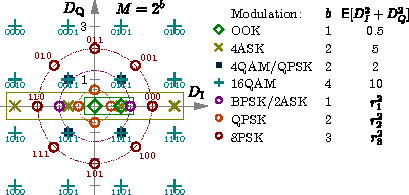
\includegraphics{./img/SK.pdf}\\
	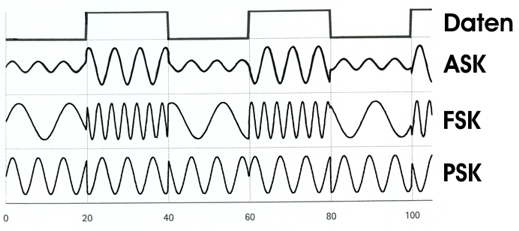
\includegraphics[width = 6cm]{./img/digimod.jpg}
}


\sectionbox{
	\subsection{On-Off Keying (OOK)}
	Intensitätsmodulation mit $b = 1$ (Laser an oder aus)\\
	Mittlere Energie pro Symbol: $E_s = $\\
}

\sectionbox{
	\subsection{Amplitude Shift Keying ($M$-ASK)}
	Für $M$ Stufen mit Abstand $\Delta$ gilt: $\E[D_I^2] = \frac{\Delta^2 (M^2-1)}{12}$
}


\sectionbox{
	\subsection{Phase Shift Keying (PSK)}
	\parbox{2.5cm}{
	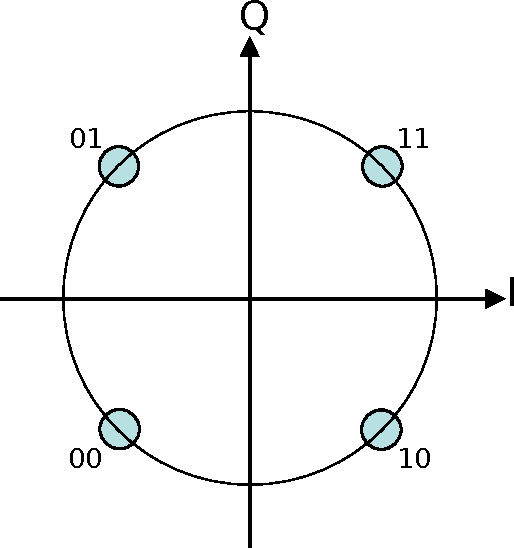
\includegraphics[width = 2.5cm]{./img/QPSK.pdf}
	} \quad 
	\parbox{4cm}{ $d_I^2 + d_Q^2 = r^2$ \qquad (meist $r = 1$) \\ $E_s = \E[D_I^2 + D_Q^2] \int_0^T \abs{g_s(t)}^2 \diff t$ \\

	Offset: verhindert harte Übergänge (Nicht durch Null)\\
	Gray-Codierung zwischen benachbarten Symbolen: Fehler in der Symbolerkennung hat nur geringe Bitfehler\\	
	}
		\subsubsection{DPSK}
		Differentielle binäre Phasenmodulation\\
		0: Phase bleibt gleich, 1: Phase ändert sich\\


}


\sectionbox{
	\subsection{Quadraturamplitudenmodulation ($M$-QAM)}
	Für $M$ Stufen und Abstand $\Delta$: $\E[D_I^2 + D_Q^2] = \frac{\Delta^2 (M-1)}{6}$
}


\vspace{0.2cm}

\raisebox{0.5cm}{Auch wichtig:} \qquad 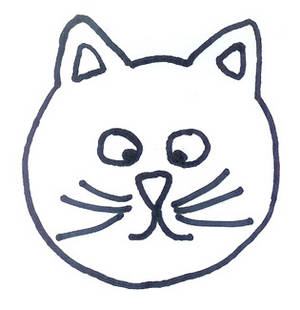
\includegraphics[height = 1cm]{./img/cat.jpg} \ \raisebox{0.5cm}{$\FT$}\ 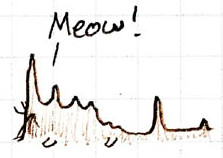
\includegraphics[height = 1.3cm]{./img/cat_f.jpg}\\
\\
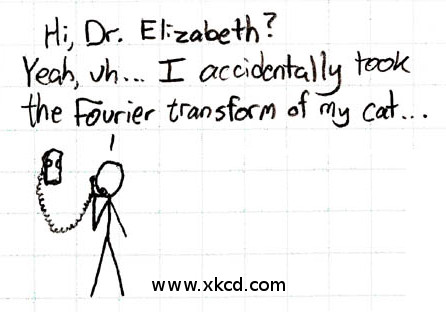
\includegraphics[width = 5cm]{./img/xkcd2.jpg}

\columnbreak
{\Huge \bf Eigene Notizen:}




% #################################################################################################################
% #################################################################################################################
\newpage
{\Huge \bf Anhang}


% SECTION ====================================================================================
\section{Mathematik}
% ============================================================================================



\sectionbox{
	\subsection{Polynome $P(x)\in\mathbb R[x]_n = \sum\limits_{i=0}^n a_ix^i$ vom Grad $n$}
	\vspace{-0.5em}
	\parbox{3cm}{ 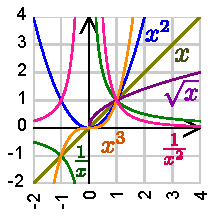
\includegraphics[scale = 0.8]{./img/math/polynome.pdf}}
	\parbox{3.5cm}{ 
	\textbf{Gerade} durch Punkt $P(x_0,y_0)$:\\[0.2em] $y = m(x - x_0) + y_0$ \\
	\\
	\textbf{Quadratisch:} $y = ax^2+bx+c$\\[0.2em]
	Mitternachtsformel für Nullstellen:\\
	\boxed{ x_{1/2}=\frac{-b\pm\sqrt{b^2-4ac}}{2a} }\\}
}

\sectionbox{
\subsection{Exponentialfunktion und Logarithmus}
\begin{tabular*}{\columnwidth}{l@{\extracolsep\fill}ll}
	$a^x = e^{x \ln a}$ & $\log_a x = \frac{\ln x}{\ln a}$ & $\ln x \le x -1$\\
	$\ln(x^{a}) = a \ln(x)$ & $\ln(\frac{x}{a}) = \ln x - \ln a$ & $\log(1) = 0$\\
\end{tabular*}
}

\sectionbox{
\subsection{Sinus, Cosinus \quad $\sin^2(x) \bs + \cos^2(x) = 1$}
\setlength{\tabcolsep}{4pt}
\tablebox{
\begin{tabular*}{\columnwidth}{@{\extracolsep\fill}c|c|c|c|c||c|c|c|c@{}} \ctrule
$x$ & $0$ & $\pi / 6$ & $\pi / 4$ & $\pi / 3$ & $\frac{1}{2}\pi$ & $\pi$ & $1\frac{1}{2}\pi$ & $2 \pi$ \\
$\scriptstyle{ \varphi }$ & $\scriptstyle{0^\circ}$ & $\scriptstyle{30^\circ}$ & $\scriptstyle{45^\circ}$ & $\scriptstyle{60^\circ}$ & $\scriptstyle{90^\circ}$ & $\scriptstyle{180^\circ}$ & $\scriptstyle{270^\circ}$ & $\scriptstyle{360^\circ}$ \\ \cmrule
$\sin$ & $0$ & $\frac{1}{2}$ & $\frac{1}{\sqrt{2}}$ & $\frac{\sqrt 3}{2}$ & $1$ & $0$ & $-1$ & $0$ \\
$\cos$ & $1$ & $\frac{\sqrt 3}{2}$ & $\frac{1}{\sqrt 2}$ & $\frac{1}{2}$ & $0$ & $-1$ & $0$ & $1$ \\     
$\tan$ & $0$ & $\frac{\sqrt{3}}{3}$ &	$1$	&	$\sqrt{3}$ & $\pm \infty$ & $0$ & $\mp \infty$ & $0$\\ \cbrule
\end{tabular*} }\\
\begin{tabular*}{\columnwidth}{@{\extracolsep\fill}ll@{}}
	Additionstheoreme &  Stammfunktionen\\
 	$\cos (x - \frac{\pi}{2}) = \sin x$ & $\int x \cos(x) \diff x = \cos(x) + x \sin(x)$\\
 	$\sin (x + \frac{\pi}{2}) = \cos x$ & $\int x \sin(x) \diff x = \sin(x) - x \cos(x)$\\
 	$\sin 2x = 2 \sin x \cos x $  & $\int \sin^2(x) \diff x = \frac12 \bigl(x - \sin(x)\cos(x) \bigr)$\\ 
 	$\cos 2x = 2\cos^2 x - 1$  & $\int \cos^2(x) \diff x = \frac12 \bigl(x + \sin(x)\cos(x) \bigr)$\\
 	$\sin(x) = \tan(x)\cos(x)$ & $\int \cos(x)\sin(x) = -\frac12 \cos^2(x)$ \\
\end{tabular*}\\[1em]
\begin{tabular*}{\columnwidth}{@{\extracolsep\fill}ll@{}}
$\sin ( x \pm y ) = \sin x \, \cos y \pm \sin y \, \cos x$ & $\sin x = \frac{1}{2 \i} (e^{\i x} - e^{- \i x })$\\
$\cos ( x \pm y ) = \cos x \, \cos y \mp \sin x \, \sin y$ & $\cos x = \frac{1}{2} (e^{\i x} + e^{- \i x })$\\
\end{tabular*}
}

\sectionbox{
	\subsection{Integralgarten}
	Partielle Integration: $\int uw'=uw-\int u'w$\\
	Substitution: $\int f(g(x)) g'(x)\,\mathrm dx=\int f(t)\, \mathrm dt$\\
	\tablebox{
	\renewcommand{\arraystretch}{1.6} 
	\begin{tabular*}{\columnwidth}{@{\hspace{5mm}}c@{\extracolsep\fill}c@{\extracolsep\fill}c@{\hspace{5mm}}} \ctrule
		$F(x) - C$ & $f(x)$ & $f'(x)$ \\ \cmrule
		$\frac{1}{q+1}x^{q+1}$ & $x^q$ & $qx^{q-1}$ \\
		\raisebox{-0.2em}{$\frac{2\sqrt{ax^3}}{3}$} & $\sqrt{ax}$ & \raisebox{0.2em}{$\frac{a}{2\sqrt{ax}}$}\\
		$x\ln(ax) -x$ & $\ln(ax)$ & $\textstyle \frac{a}{x}$\\
		%e^x & e^x & e^x \\
		$\frac{1}{a^2} e^{ax}(ax- 1)$ & $x \cdot e^{ax}$ & $e^{ax}(ax+1)$ \\
		$\frac{a^x}{\ln(a)}$ & $a^x$ & $a^x \ln(a)$ \\
		$-\cos(x)$ & $\sin(x)$ & $\cos(x)$\\
		$\cosh(x)$ & $\sinh(x)$ & $\cosh(x)$\\
		$\mathrm{Si}(x)$ & $\sinc(x)$ & $\frac{x \cos(x) - \sin(x)}{x^2}$\\
		$-\ln |\cos(x)|$ & $\tan(x)$ & $\frac{1}{\cos^2(x)}$ \\ \cbrule
	\end{tabular*} }\\
	$\int e^{at} \sin(bt) \diff t = e^{at} \frac{a \sin(bt) + b \cos(bt)}{a^2 + b^2}$\\
	\begin{tabular*}{\columnwidth}{@{\extracolsep\fill}ll@{}}
	$\int x e^{ax^2} \diff x = \frac{1}{2a} e^{ax^2}$ & $\int t^2 e^{at} \diff t = \frac{(ax-1)^2+1}{a^3} e^{at}$\\
	\end{tabular*} 
}

\begin{tabular}{llllllllllll}
	$2^1$ & $2^2$ & $2^3$ & $2^4$ & $2^5$ & $2^6$ & $2^7$ & $2^8$ & $2^{16}$\\ \mrule
	2 & 4 & 8 & 16 & 32 & 64 & 128 & 256 & 65536\\
\end{tabular}


% SECTION ====================================================================================
\section{Geometrie \qquad $a^2 + b^2 = c^2$}
% ============================================================================================
\sectionbox{
\begin{tabular*}{\columnwidth}{@{\extracolsep\fill}ll@{}}
	\pbox{4cm}{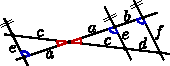
\includegraphics{./img/math/strahlensatz.pdf} } &
	\pbox{8cm}{
	\textbf{Strahlensatz:}\\[0.2em]
	%\begin{tabular}{@{}ll}
	\large $a:b = c:d$ \quad \Large $\frac{a+b}{c+d} = \frac{a}{c} = \frac{b}{d}$\\[0.3em]
	\Large $\frac{a}{a+b} = \frac{c}{c+d} = \frac{e}{f}$}\\
\end{tabular*}\\
\\
Innenwinkelsumme im $n$-Eck: $(n-2) \cdot 180^\circ$\\
\\
\textbf{Allg. Dreieck} $\triangle ABC$ mit Seiten $a,b,c$ und Winkel $\alpha,\beta,\gamma$:\\[0.2em]
\begin{tabular*}{\columnwidth}{@{\extracolsep\fill}lll@{}}
	\multirow{3}{1.6cm}{ 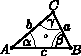
\includegraphics{./img/math/dreieck.pdf} } & Kosinussatz: & $ c^2 = a^2 + b^2 - 2ab \cos(\gamma)$\\[0.2em]
	& Sinussatz: & $\frac{a}{\sin \alpha} = \frac{b}{\sin \beta} = \frac{c}{\sin \gamma}$ \\[0.2em]
	& Projektionssatz: & $c = a \cos \beta + b \cos \alpha$ \\
\end{tabular*}\\
	Höhe $h_c = a \sin \beta = b \sin \alpha$  \qquad Fläche $A = \frac{1}{2} h_c c = \frac{1}{2} h_a a$\\
	Schwerpunkt: $x_S = \frac{1}{3}(x_A + x_B + x_C)$ \quad $y_S = \frac{1}{3}(y_A + y_B + y_C)$\\ 
\\[1em]
\textbf{Rechtwinkliges Dreieck} $\triangle ABC$ mit $\gamma = 90^\circ$ bei $C$\\[0.2em]
	\begin{tabular}{@{}lll}
	\multirow{3}{2cm}{ 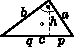
\includegraphics[scale = 1.4]{./img/math/rechtwinklig.pdf} } & Pythagoras: & \hspace{-2.5mm} \large $a^2 + b^2 = c^2$\\[0.1em]
	& Höhensatz: & \hspace{-2.5mm} {\large $h^2 = pq$}\\[0.1em]
	& Kathetensatz: & \hspace{-2.5mm} \large $a^2 = pc$\\[0.1em]
	& \multicolumn{2}{l}{\large $a = c \sin \alpha = c \cos \beta = b \tan \alpha$}\\ 
\end{tabular}\\
\\[1em]
\pbox{5cm}{
\textbf{Pyramide} mit beliebiger Grundfläche $G$\\
\begin{tabular}{@{}ll}
	\multirow{2}{0.8cm}{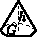
\includegraphics{./img/math/pyramide.pdf} } & $V = \frac{1}{3} G \cdot h$\\
	& SP: liegt auf $h$ mit $y_S = h/4$\\
\end{tabular} } \qquad
\pbox{3cm}{
\textbf{Zylinder/Prisma}\\[0.3em]
$V = G \cdot h$\\[0.2em]
$M = U \cdot h$\\
}\\
\\ \\
\pbox{1.0cm}{ 
\includegraphics{./img/math/kreis.pdf} } \qquad
\parbox{4cm}{
\begin{tabular}{lll}
\textbf{Kreis:} & $A = \pi r^2$ & $U =2\pi r$ \\ 
\textbf{Kugel:} & $V = \frac{4}{3} \pi r^3$ & $O = 4 \pi r^2$\\
\end{tabular} }


Kreissehne: $s = 2r \sin(\alpha/2)$
}


% SECTION ====================================================================================
\section{Stochastik}
% ============================================================================================
\sectionbox{
\subsection{Der Wahrscheinlichkeitsraum $(\Omega,\mathbb F,\P)$}
Ein Wahrscheinlichkeitsraum $(\Omega,\mathbb F,\P)$ besteht aus\\
\begin{tabular*}{\columnwidth}{@{\extracolsep\fill}lll@{}} \ctrule
\textbf{Ergebnismenge} & $\Omega = \eset{\omega_1,\omega_2, ...}$ & Ergebnis $\omega_j \in \Omega$\\[0.5em]
\textbf{Ereignisalgebra} & $\mathbb F = \eset{A_1,A_2,...}$ & Ereignis $A_i \subseteq \Omega$\\
\textbf{Wahrscheinlichkeitsmaß} & $\P:\mathbb F \ra [0,1]$ & $\P(A) = \frac{|A|}{|\Omega|}$\\ \cbrule
\end{tabular*}

Es gilt: $\P(A \cup B) = \P(A) + \P(B) - \P(A \cap B)$\\ \\
\textbf{Bedingte Wahrscheinlichkeit} für $A$ falls $B$ bereits eingetreten ist:\\
$\P_B(A) = \P(A|B) = \frac{\P(A \cap B)}{\P(B)}$\\
Multiplikationssatz: $\P(A \cap B) = \P(A|B)\P(B) = \P(B|A)\P(A)$\\
\\
\textbf{Erwartungswert:} $\E[X] = \mu = \sum x_i P(x_i) = \int \limits_\mathbb R x \cdot f_{\X} (x) \diff x$ \\ 
\textbf{Varianz:} $\Var [X] = \E \big[(\X - \E[\X])^2\big] = \E[\X^2] - \E[\X]^2$\\
Standard Abweichung $\sigma = \sqrt{\Var[\X]}$\\
\\
\textbf{Covarianz:} $\Cov [\X,\Y] = \E[(\X- \E[\X])(\Y - \E[\Y])] = \Cov [\Y, \X]$\\
\\
	\textbf{Binominialverteilung} (diskret, $n$ Versuche, $k$ Treffer): \\
	$P(X=k)= \binom nk p^k (1-p)^{n-k}$ \quad $\mu = np$ \quad $\sigma^2 = np(1-p)$\\

	\textbf{Korrelation} ist ein Maß für den linearen Zusammenhang von Variablen\\
	Kreuzkorrelation von $\X$ und $\Y$: \boxed{ r_{xy} = \frac{\Cov(\X, \Y)}{\sigma_{\X} \sigma_{\Y}} }\\	
}

\sectionbox{
	\subsection{Normalverteilung}

	\textbf{PDF:} \boxed{f_X (x) = \frac{1}{\sqrt{2 \pi \sigma^2}} e^{-\frac{(x-\mu)^2}{2 \sigma^2}} \quad x \in \mathbb R}\\
	\tablebox{ \everymath{\displaystyle}
		\begin{tabular*}{\columnwidth}{l@{\extracolsep\fill}ll} \ctrule
			$\underset{\text{Erwartungswert}}{\E(\X) = \mu}$ & $\underset{\text{Varianz}}{\Var(\X) =\sigma^2}$ & $\underset{\text{Charakt. Funktion}}{\varphi_{\X}(\omega) = e^{j\omega\mu-\frac{\omega^2\sigma^2}{2}}}$\\ \cbrule
		\end{tabular*} \everymath{\textstyle} }
}


% SECTION ====================================================================================
\section{Signale}
% ============================================================================================


\sectionbox{
	\subsection{Faltung von Signalen}
	\emphbox{ $\displaystyle x(t) * h(t) = h(t) * x(t) = \int\limits_{-\infty}^{\infty} x(\tau) \cdot h(t-\tau) \diff \tau$ }

	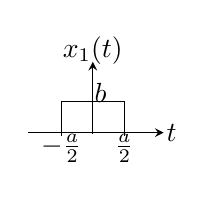
\begin{tikzpicture}[scale=0.2]
		% Gitter zeichnen
		%\draw[help lines] (-4,0) grid (4,4);
		
		% Koordinatenachsen zeichnen
		\begin{scope}[>=stealth]
			\draw[->] (-4.1,0) to (4.5,0);
			\draw[->] (0,-0.1) to (0,4.5);
		\end{scope}
		
		% Achsenbeschriftungen eintragen
		\node (t-Axis) at (5,0) {$t$};
		\node (x-Axis) at (0,5.2) {$x_1(t)$};
		
		% Graph zeichnen
		\draw plot coordinates {(-2,0) (-2,2) (2,2) (2,0)};
		
		% Achsenmarkierungen
		\draw (-2,-0.2) to (-2,0.2);
		\draw (2,-0.2) to (2,0.2);
		\draw (-0.2,2) to (0.2,2);
		\node at (-2,-1) {$-\frac{a}{2}$};
		\node at (2,-1) {$\frac{a}{2}$};
		\node at (0.5,2.5) {$b$};
	\end{tikzpicture}
	\raisebox{0.8cm}{$*$}
	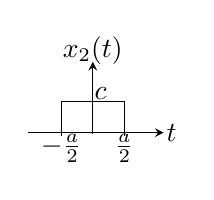
\begin{tikzpicture}[scale=0.2]
			% Gitter zeichnen
			%\draw[help lines] (-4,0) grid (4,4);
			
			% Koordinatenachsen zeichnen
			\begin{scope}[>=stealth]
				\draw[->] (-4.1,0) to (4.5,0);
				\draw[->] (0,-0.1) to (0,4.5);
			\end{scope}
			
			% Achsenbeschriftungen eintragen
			\node (t-Axis) at (5,0) {$t$};
			\node (x-Axis) at (0,5.2) {$x_2(t)$};
			
			% Graph zeichnen
			\draw plot coordinates {(-2,0) (-2,2) (2,2) (2,0)};
			
			% Achsenmarkierungen
			\draw (-2,-0.2) to (-2,0.2);
			\draw (2,-0.2) to (2,0.2);
			\draw (-0.2,2) to (0.2,2);
			\node at (-2,-1) {$-\frac{a}{2}$};
			\node at (2,-1) {$\frac{a}{2}$};
			\node at (0.5,2.5) {$c$};
	\end{tikzpicture}
	\raisebox{0.8cm}{$=$}
	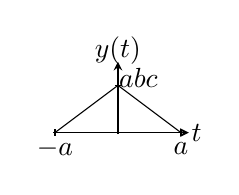
\begin{tikzpicture}[scale=0.2]
			% Gitter zeichnen
			%\draw[help lines] (-4,0) grid (4,4);
			
			% Koordinatenachsen zeichnen
			\begin{scope}[>=stealth]
				\draw[->] (-4.1,0) to (4.5,0);
				\draw[->] (0,-0.1) to (0,4.5);
			\end{scope}
			
			% Achsenbeschriftungen eintragen
			\node (t-Axis) at (5,0) {$t$};
			\node (x-Axis) at (0,5.2) {$y(t)$};
			
			% Graph zeichnen
			\draw plot coordinates {(-4,0) (0,3) (4,0)};
			
			% Achsenmarkierungen
			\draw (-4,-0.2) to (-4,0.2);
			\draw (4,-0.2) to (4,0.2);
			\draw (-0.2,3) to (0.2,3);
			\node at (-4,-1) {$-a$};
			\node at (4,-1) {$a$};
			\node at (1.3,3.5) {$abc$};
	\end{tikzpicture}


$\sinc\left(\frac{t}{T_A}\right) * \sinc\left(\frac{t}{T_A}\right) = T_A \sinc\left(\frac{t}{T_A}\right)$

}

\sectionbox{
	\subsection{sinc-Singal}
	\pbox{4.8cm}{
	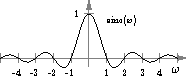
\includegraphics[scale = 1.3]{./img/sinc.pdf}
	}
	\pbox{2.0cm}{$\sinc(x) = \frac{\sin(\pi x)}{\pi x}$ \\ $ = \mathrm{si}(\pi x)$ \\ \\ 
	 FT: \\ $\sinc(t) \FT \rect(f)$}

}



% SECTION ====================================================================================
\section{Fouriertransformation}
% ============================================================================================

\emphbox{ $\displaystyle \underset{\text{Zeitbereich}}{\large x(t)} \FT \underset{\text{Frequenzspektrum}}{\large X(f)} := \int\limits_{-\infty}^\infty x(t) \exp(-\j 2 \pi f t) \diff t$ }

\sectionbox{
	\subsection{Eigenschaften der Fouriertrafo}
	\tablebox{
	\begin{tabular*}{\columnwidth}{@{\extracolsep\fill}ll@{}}
	\ctrule 
	Linearität: & $\alpha x(t) + \beta g(t) \FT \alpha X(f) + \beta G(f)$\\
	Zeitverschiebung: & $x(t - \tau) \FT e^{- \j 2\pi f \tau} X(f)$\\
	Frequenzversch. & $e^{\j 2 \pi f_0 t} \FT X(f - f_0)$\\
	Vertauschung: & $U^* (t) \FT u^* (f)$ \\ 
	Stauchung & $x(ct) \FT \frac{1}{\abs{c}} X\bigl(\frac{f}{c}\bigr)$\\
	Ableitung & $x^{(n)}(t) \FT (\j 2 \pi f)^n X(f)$\\
	Integral & $\int_{-\infty}^t x(\tau) \diff \tau \FT \left(\frac{1}{2}\dirac(f) - \frac{\j}{2 \pi f}\right) X(f)$\\
	Faltung: & $(x * g)(t) \FT X(f) \cdot G(f)$\\
	Parseval: & $\int \limits_{-\infty}^{+\infty} u_1 (t) \cdot u_2^* (t) \diff t = \int \limits_{-\infty}^{+\infty} U_1 (f) \cdot U_2^* (f) \diff f$ \\
	Energie: & $E = \int \limits_{-\infty}^{+\infty} \abs{u(t)}^2 \diff t = \int \limits_{-\infty}^{+\infty} \abs{U(f)}^2 \diff f$ \\ 
	\cbrule
	\end{tabular*}
}
\\ 
	Zusammenhang zwischen geraden und ungeraden Signalanteilen:
	\begin{center}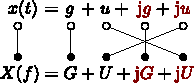
\includegraphics[height=1.5cm]{./img/FT/FT.pdf}\end{center}

	$x(t) \FT X(f) \FT x(-t) \FT X(- f)$\\
	Bei periodischen Signalen: Fourierreihen!
}


% ======================================================================
\columnbreak
\sectionbox{
	\subsection{Wichtige Fouriertransformationen}

	\begin{tabular*}{\columnwidth}{c@{\extracolsep\fill}c}
		\large Zeitfunktion & \large Spektrum\\ \mrule
		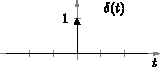
\includegraphics{./img/FT/dirac_t.pdf} & 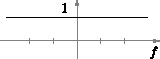
\includegraphics{./img/FT/dirac_f.pdf}\\[1em]
		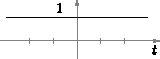
\includegraphics{./img/FT/1_t.pdf} & 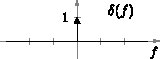
\includegraphics{./img/FT/1_f.pdf}\\[1em]
		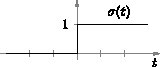
\includegraphics{./img/FT/sigma_t.pdf} & 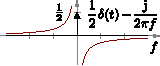
\includegraphics{./img/FT/sigma_f.pdf}\\[1em]
		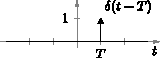
\includegraphics{./img/FT/verschiebung_t.pdf} & 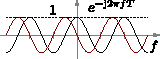
\includegraphics{./img/FT/verschiebung_f.pdf}\\[1em]
		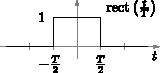
\includegraphics{./img/FT/rect_t.pdf} &  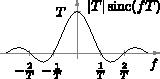
\includegraphics{./img/FT/rect_f.pdf}\\[1em]
		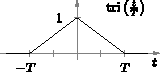
\includegraphics{./img/FT/tri_t.pdf} & 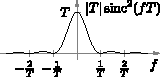
\includegraphics{./img/FT/tri_f.pdf}\\[1em]
		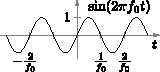
\includegraphics{./img/FT/sin_t.pdf} & 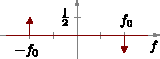
\includegraphics{./img/FT/sin_f.pdf}\\[1em]
		\includegraphics{./img/FT/cos_t.pdf} & \includegraphics{./img/FT/cos_f.pdf}\\[1em]
		\includegraphics{./img/FT/dirac_folge_t.pdf} & \includegraphics{./img/FT/dirac_folge_f.pdf}\\[1em]
	\end{tabular*}


%	Verschiedene Normungen:\\
%	\begin{tabular}{@{}ll}
%		Norm $1$: &$x(t) \FT X(\omega) \FT 2 \pi x(-t) \FT 2 \pi X(- \omega)$\\
%		Norm $\frac{1}{\sqrt{2 \pi}}$: & $x(t) \FT X(\omega) \FT x(-t) \FT X(- \omega)$\\
%	\end{tabular}

}


\sectionbox{
	\subsection{Weitere Paare}
\tablebox{
	\begin{tabular*}{\columnwidth}{@{\extracolsep\fill}cc | cc@{}}
	\ctrule
		$f(t)$ 					& $F(\omega)$									& $f(t)$		 						& $F(\omega)$\\	
		\cmrule		
		$|t^n|$ 				&  $\frac{2n!}{(\i \omega)^{n+1}}$				& $\sinc(\frac{t}{T})$					& $T \rect(fT)$\\
		$t^n$ 					& $2\pi \i^n \delta^{(n)}(\omega)$ 				& $\frac{t^{n-1}}{(n-1)!} e^{-at} u(t)$ & $\frac{1}{(a+\i \omega)^n}$\\[0.5em]
								& 												& $\exp(-\alpha t)$		& $\frac{1}{\i 2 \pi f + \alpha}$ \\
		\cbrule
	\end{tabular*}
	}
}



% Ende der Spalten
\end{multicols*}

% Dokumentende
% ======================================================================
\end{document}

% ToDos:




	\begin{align*}
		f(t) 					& \FT F(\omega) 						& f(t) 						& \FT F(\omega)\\
		1 						& \FT 2\pi \delta(\omega)				& \delta(t-t_0) 			& \FT e^{-\i \omega t_0}\\
		\heavi(t) 				& \LT \frac{1}{\i \omega} + \pi \delta(\omega) & t \heavi(t)		& \FT \\
		|t^n| 					& \FT \frac{2n!}{(\i \omega)^{n+1}}\\
		\tri(\frac{t}{T}) 		& \FT T \sinc^2(\omega T)		& \rect(\frac{t}{2T})		& \FT 2T \sinc(\omega T) \\
	\end{align*}
